\documentclass{scrreprt}
\usepackage[utf8]{inputenc}
\usepackage[english]{babel}
\usepackage{graphicx}
\usepackage{tabularx}
\usepackage{booktabs}
\usepackage{amsmath}
\usepackage{float}
\usepackage[margin=2.5cm]{geometry}
\usepackage[bookmarks=true]{hyperref}

\hypersetup{
    bookmarks=false,
    pdftitle={Software Requirements Specification - ProjNaN},
    pdfauthor={Vanshaj Sharma, Aryan Thakkar},
    pdfsubject={Software Requirements Specification},
    pdfkeywords={SRS, ProjNaN, Project Management, Contribution Verification, GitHub},
    colorlinks=true,
    linkcolor=blue,
    citecolor=black,
    filecolor=black,
    urlcolor=purple,
    linktoc=page
}

\def\myversion{1.0}

\begin{document}

%% TITLE PAGE
\begin{titlepage}
\begin{flushright}
    \rule{\linewidth}{4pt}\vskip0.8cm
    \begin{bfseries}
        \Huge{SOFTWARE REQUIREMENTS\\ SPECIFICATION}\\[0.6cm]
        \Large{for}\\[0.6cm]
        \Huge{ProjNaN}\\[0.3cm]
        \large{An Educational Collaborative Project Management\\ and Contribution Verification Platform}\\[0.8cm]
        \LARGE{Version \myversion}\\[0.9cm]
        \normalsize
        Prepared by:\\[0.2cm]
        Vanshaj Sharma (Roll No: 1024160114)\\
        Aryan Thakkar (Roll No: 1024160100)\\[0.4cm]
        Group: 3P14, BE Third Year, COSE\\[0.8cm]
        Submitted to:\\[0.2cm]
        Dr. Anushka\\
        Assistant Professor\\
        Computer Science and Engineering Department\\
        Thapar Institute of Engineering and Technology, Patiala\\[0.8cm]
        Course: UCS 503 -- Software Engineering\\[0.8cm]
        October 15, 2026
    \end{bfseries}
\end{flushright}
\end{titlepage}

\tableofcontents

%% CHAPTER 1: INTRODUCTION
\chapter{Introduction}\label{chap:introduction}

\section{Purpose}\label{sec:purpose}
In university computer science courses, Project-Based Learning is a core teaching method. Students collaborate in small teams to design and build software systems over a semester. However, evaluating collaborative student projects is difficult for course instructors. Traditional grading relies on periodic milestone presentations, written status reports, or final compressed code archives. These methods give teachers little direct visibility into individual participation, code authorship regularity, or task authenticity. Often, a few active students do most of the work while others contribute very little (social loafing or free-riding).

ProjNaN is an educational project management and contribution verification web platform built to solve this problem. ProjNaN connects classroom administration (teachers, classes, student teams) with modern version control activity from GitHub (commits, pull requests, and issues). By combining interactive Kanban task boards with repository tracking and an internal rule-based verification engine, ProjNaN provides an authentic, transparent record of each student's technical contributions.

\section{Intended Audience and Reading Suggestions}\label{sec:audience}
This Software Requirements Specification (SRS) is intended for course instructors, student developers, academic evaluators, software architects, and quality assurance testers. It describes the complete functional requirements, system behavior, user roles, technical environment, and nonfunctional qualities of ProjNaN.

Readers interested in the overall concept and user roles should review Chapters 1 and 2. Developers and testers should examine the detailed functional requirements in Chapter 3 and nonfunctional constraints in Chapter 4. Maintenance and future extensions are outlined in Chapter 5.

\section{Project Scope}\label{sec:scope}
ProjNaN provides an academic workspace tailored for university courses. Instructors create academic classes, generate unique join codes, and supervise student teams. Students enroll in classes, form teams, organize tasks on a Kanban board, and link their team's remote GitHub repository.

When a student finishes an assigned task, they submit completion evidence such as pull request citations, commit hashes, and descriptive notes. An internal deterministic rule-based evaluation engine checks the submitted evidence against synchronized repository records and assigns an assistive confidence score ($0.20 - 0.98$). Course instructors hold final verification authority: approving a task awards gamified Experience Points (XP) to the student and records an immutable entry in the project contribution ledger, while rejecting a task returns it to the student with feedback for revision.

\begin{figure}[H]
    \centering
    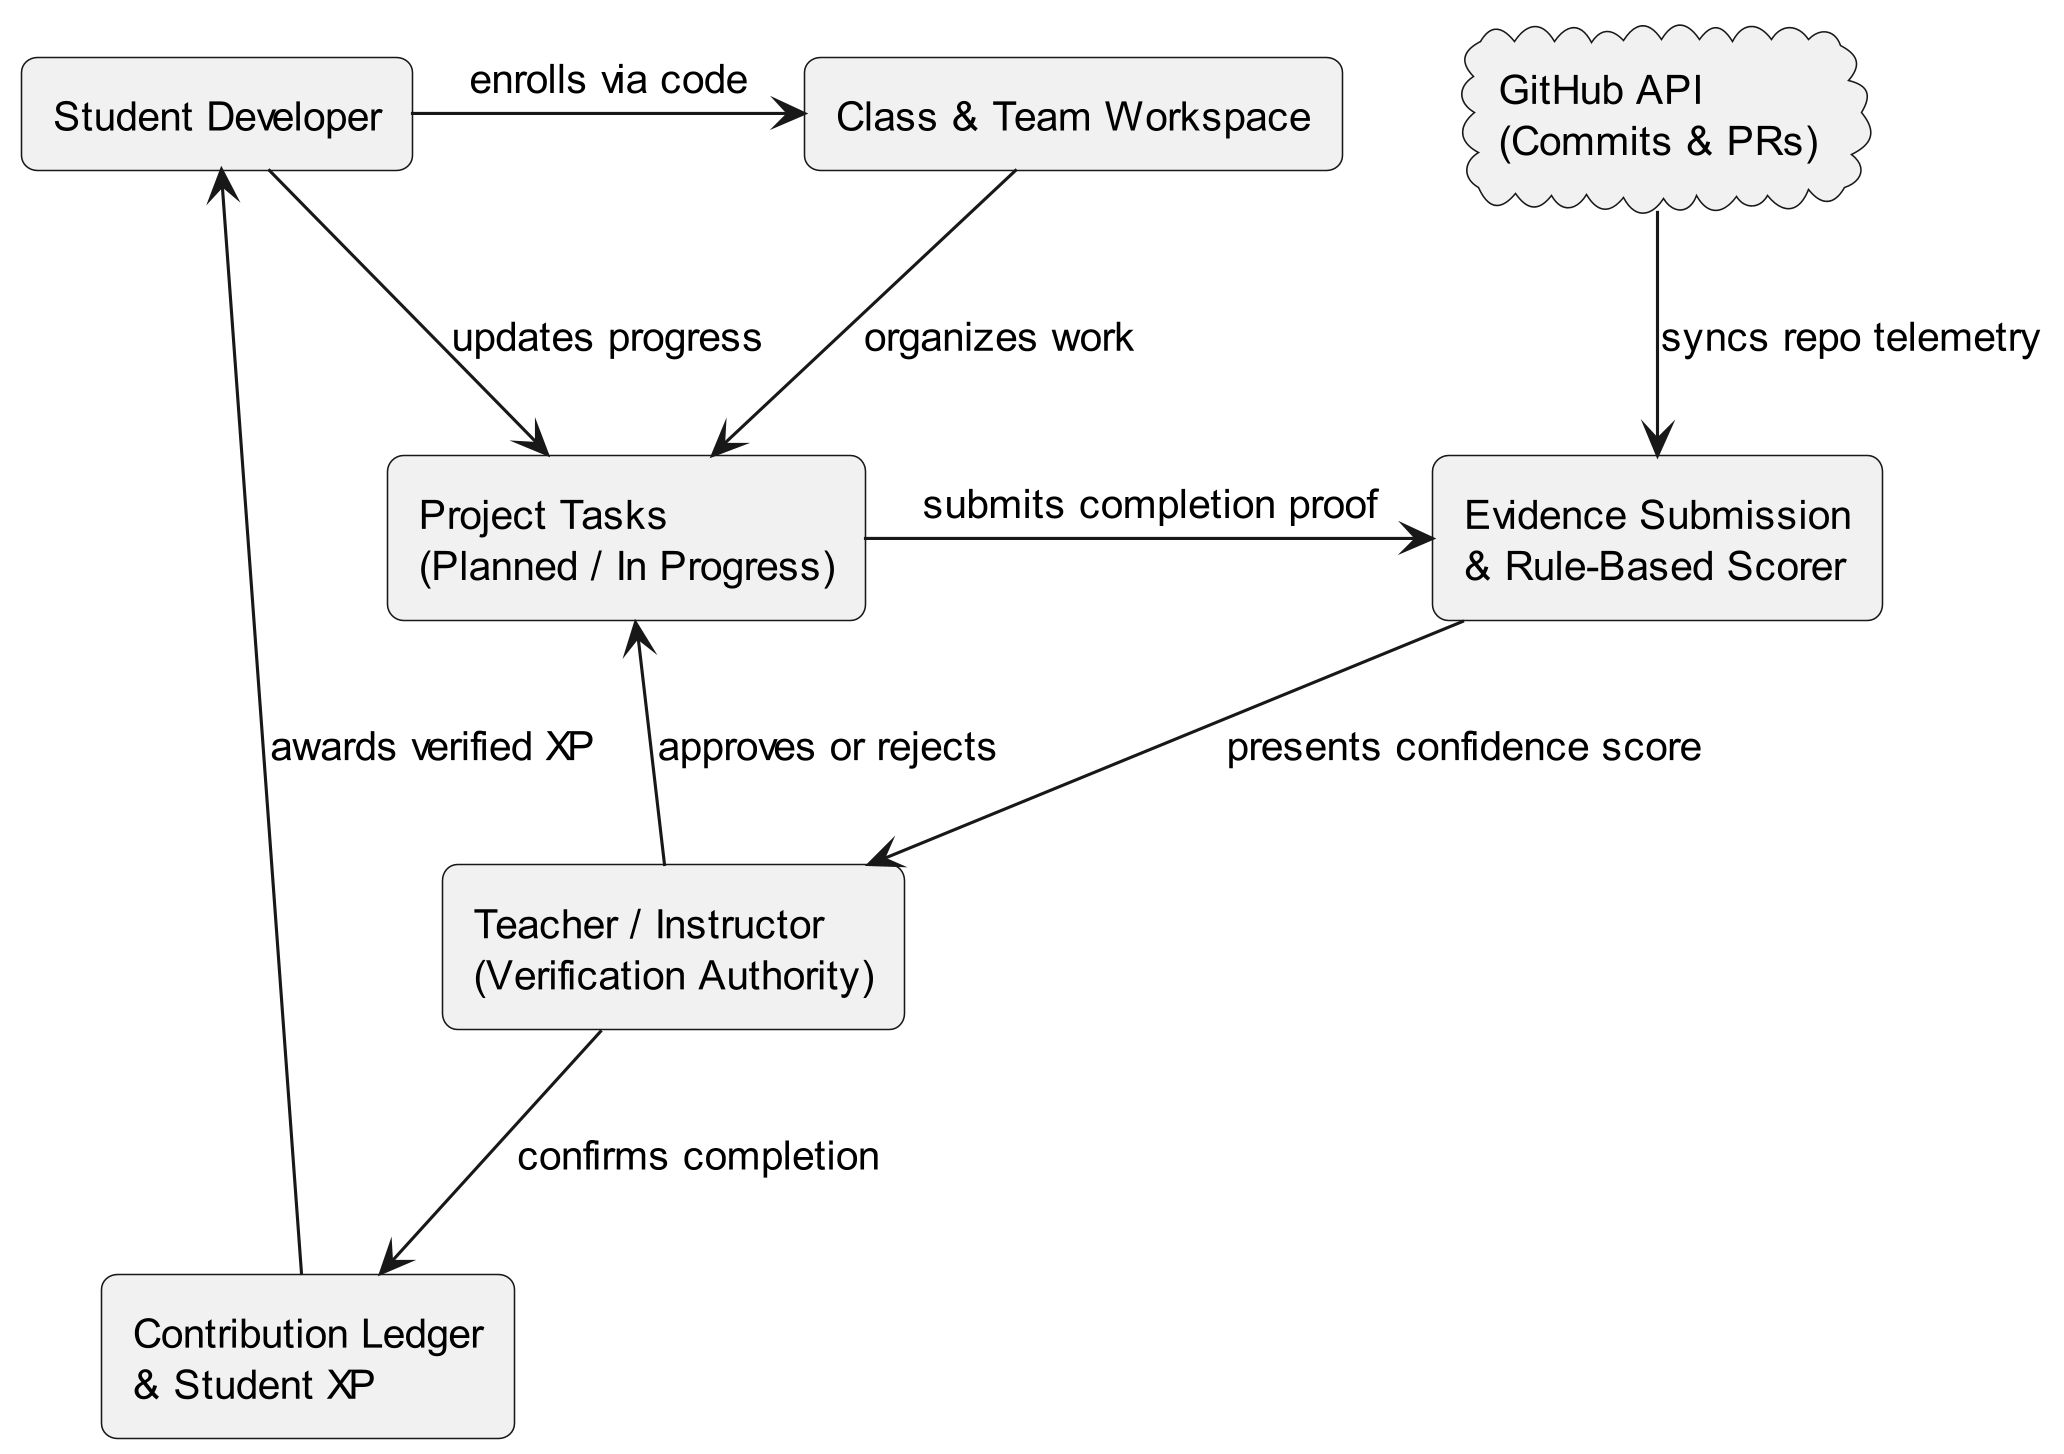
\includegraphics[width=0.88\textwidth]{workflow.png}
    \caption{Overall Workflow of the ProjNaN Platform}
    \label{fig:overall_workflow}
\end{figure}

Figure~\ref{fig:overall_workflow} illustrates the overall workflow of ProjNaN across two interacting cycles:
\begin{itemize}
    \item \textbf{Student Cycle}: Students enroll in classes using unique join codes, form collaborative teams, and create discrete tasks. While implementing features, they commit code to GitHub, submit completion evidence on ProjNaN, and receive verified XP upon instructor approval.
    \item \textbf{Teacher Cycle}: Teachers establish course sections, supervise project teams, inspect student completion evidence alongside rule-based confidence scores, make authoritative verification decisions, and review relative effort distribution across team members.
\end{itemize}


%% CHAPTER 2: OVERALL DESCRIPTION
\chapter{Overall Description}\label{chap:overall_description}

\section{Product Perspective}\label{sec:product_perspective}
ProjNaN is an independent, self-contained web platform designed to replace manual, unverified project grading. Commercial project management tools (such as Jira or Trello) are built for enterprise software teams; they lack academic course hierarchies, peer accountability mechanisms, and instructor verification gates. Conversely, standard learning management systems track grades but have no connection to version control systems where students actually write code.

ProjNaN bridges this gap. It acts as an educational project management system that combines course rosters and team workspaces with automated GitHub telemetry ingestion, rule-based verification pre-scoring, and an idempotent contribution accounting ledger.

\section{User Classes and Characteristics}\label{sec:user_classes}
ProjNaN serves two primary in-application user roles:

\begin{itemize}
    \item \textbf{Course Instructor (Teacher)}: Academic faculty members who create classes, distribute join codes, set milestones, inspect student evidence, approve or reject task verifications, submit qualitative evaluations (1--5 star reviews), and review team contribution analytics.
    \item \textbf{Student Developer (Student)}: Enrolled undergraduate students who join classes using class codes, organize into project teams, create and claim Kanban tasks, submit technical evidence, complete weekly arena coding challenges, and track their earned XP and velocity.
\end{itemize}

In addition, two specialized operational responsibilities exist within the system:
\begin{itemize}
    \item \textbf{Student Team Leader}: An enrolled student designated as team leader who holds the additional responsibility of linking the team's remote GitHub repository and coordinating milestone target dates. This is an operational responsibility, not a separate application role.
    \item \textbf{Infrastructure Administrator}: A DevOps or system administrator operating strictly at the host server infrastructure layer (server provisioning, SQLite backups, environment variables). This actor does not participate as an in-app user.
\end{itemize}

\begin{figure}[H]
    \centering
    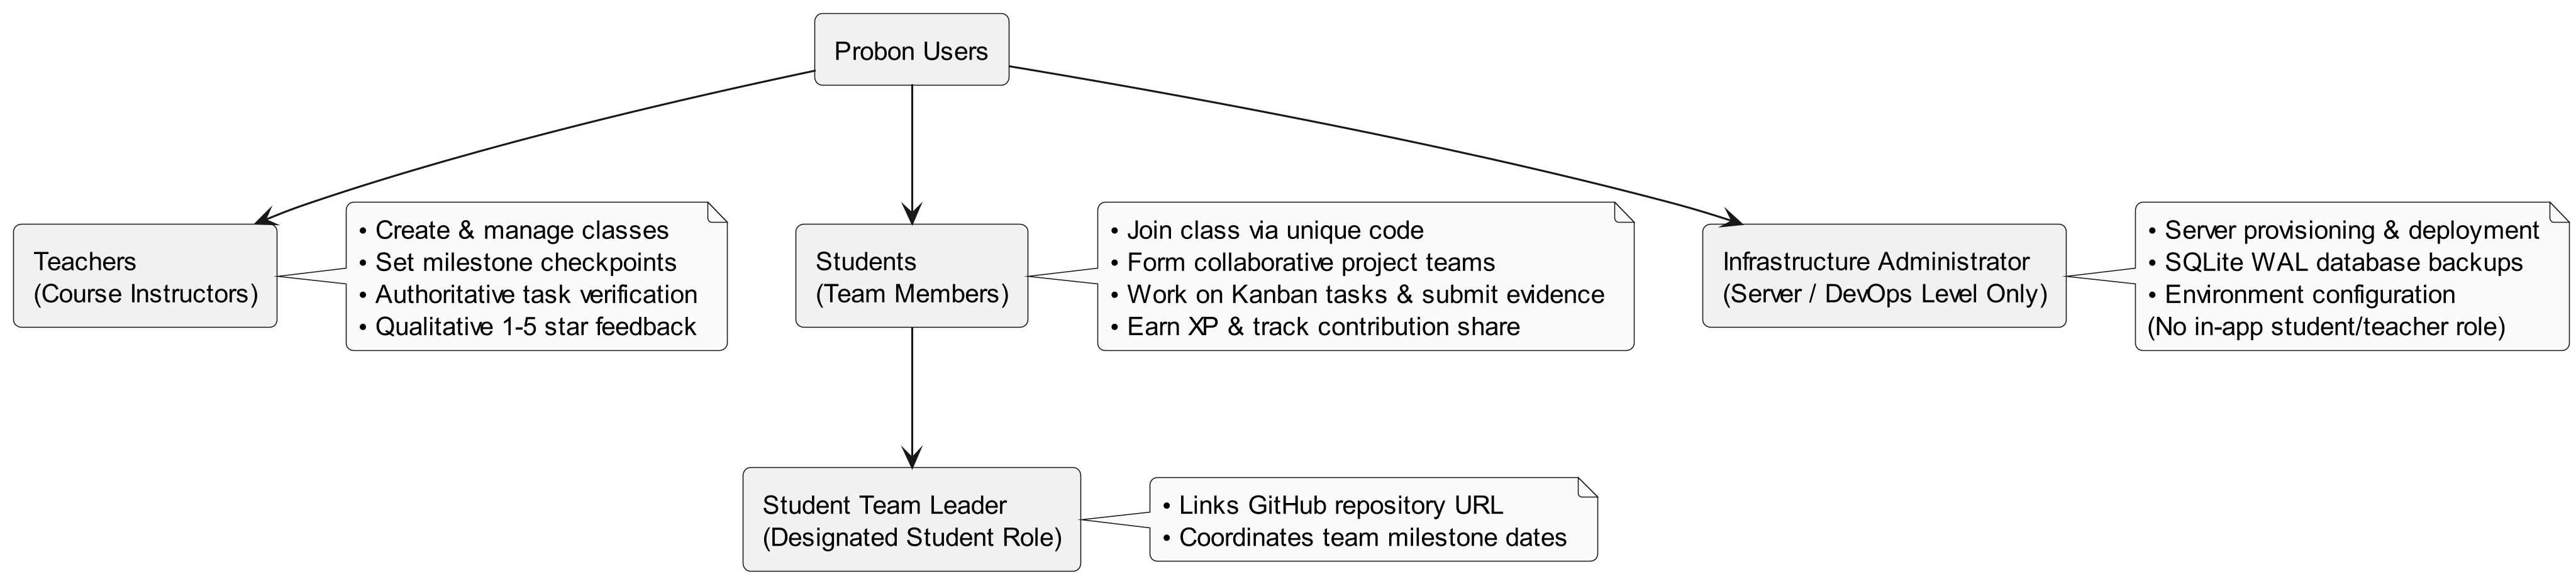
\includegraphics[width=0.95\textwidth]{user_types.png}
    \caption{ProjNaN User Hierarchy and Operational Responsibilities}
    \label{fig:user_types}
\end{figure}

\section{Product Functions}\label{sec:product_functions}
The primary functions of ProjNaN include:
\begin{enumerate}
    \item \textbf{Authentication and Access Control}: Student and teacher registration, secure password hashing with bcrypt, stateless session management using JSON Web Tokens (JWT), email verification tokens, and password reset workflows.
    \item \textbf{Academic Hierarchy and Team Scoping}: Teacher-managed class sections, unique collision-resistant join codes, student self-enrollment, team formation, and roster visibility.
    \item \textbf{Project Workspaces and Milestones}: Dedicated team project spaces, milestone target dates, and automated dynamic progress percentage calculations.
    \item \textbf{4-Stage Task State Machine}: Structured task lifecycle transitions (\texttt{Planned} $\rightarrow$ \texttt{In Progress} $\rightarrow$ \texttt{Verification Pending} $\rightarrow$ \texttt{Completed}) preventing arbitrary student self-completion.
    \item \textbf{Heuristic Evidence Evaluation}: Rule-based pattern matching and repository cross-referencing that generates an assistive confidence score ($0.20 - 0.98$) for instructor review.
    \item \textbf{Authoritative Faculty Verification}: Instructor approval or rejection of submitted tasks, ensuring only verified work earns gamified XP and contribution points.
    \item \textbf{GitHub Telemetry Synchronization}: Background ingestion of remote Git commits, pull requests, and issues from the GitHub REST API v3 into local storage.
    \item \textbf{Idempotent Contribution Ledger and Team Analytics}: Unique contribution keys preventing duplicate credit, individual effort share calculations ($P_i$), and rolling 14-day velocity sparklines.
    \item \textbf{Gamification and Weekly Arena}: Difficulty-tiered coding challenges, achievement badges, and student rank progression from Novice to Master.
    \item \textbf{Pedagogical Feedback}: Structured 1--5 star instructor ratings and qualitative reviews.
    \item \textbf{Persistent Notifications and Channels}: Event-driven alert badges and project discussion channels.
\end{enumerate}

\clearpage
\begin{figure}[H]
    \centering
    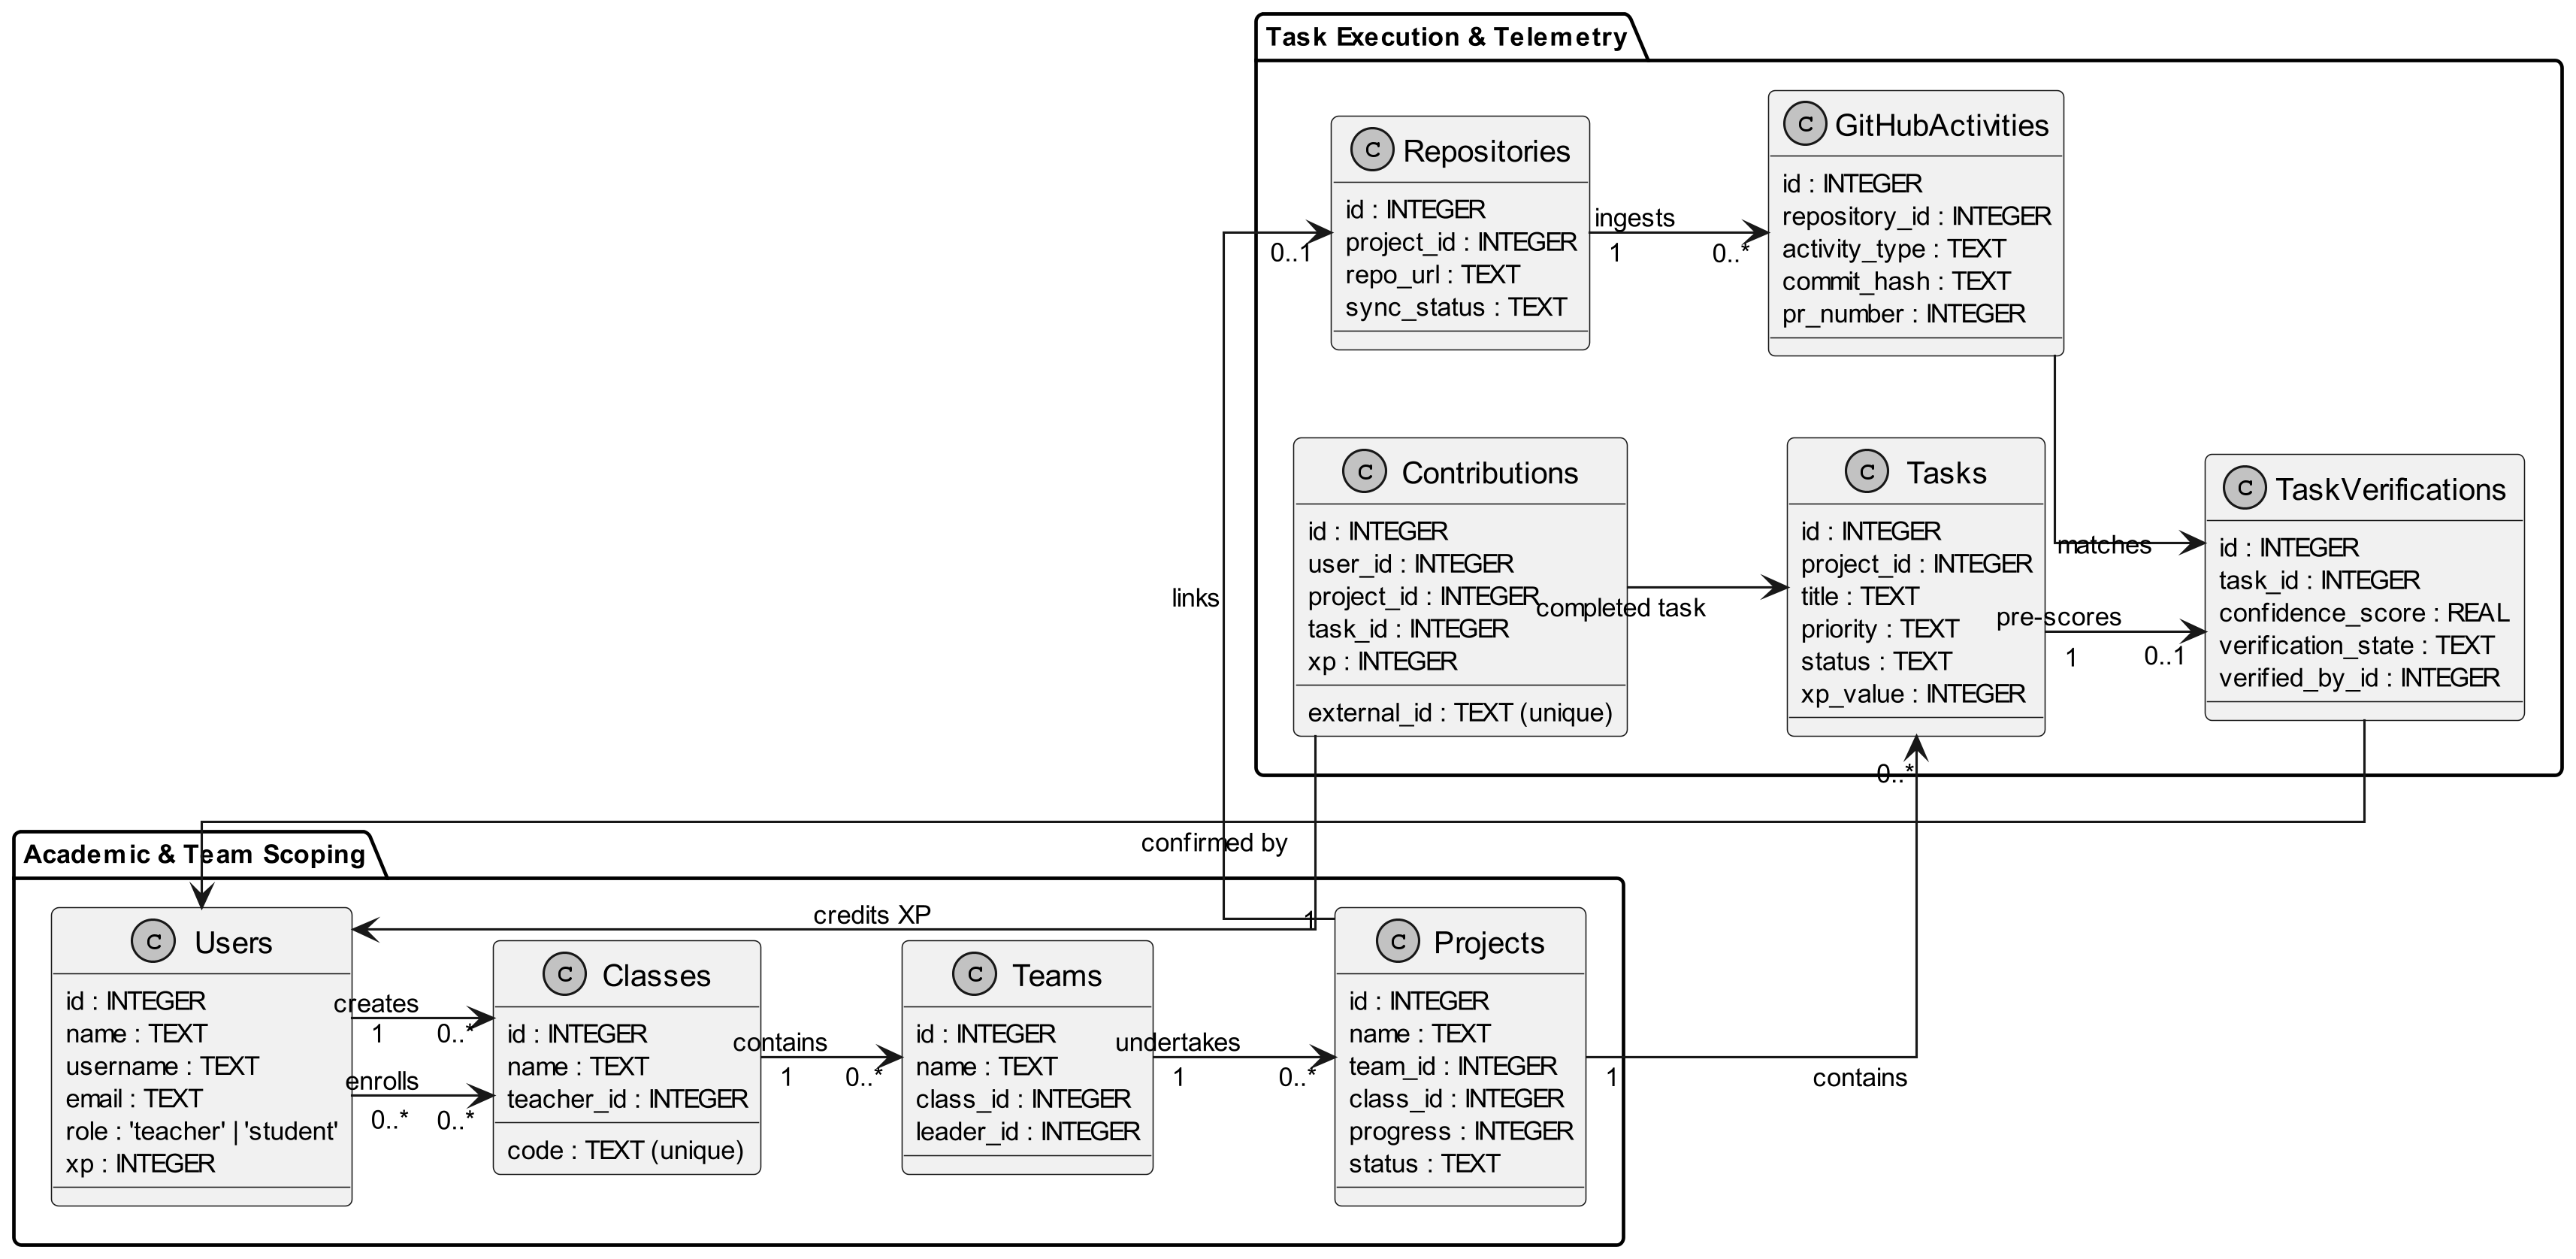
\includegraphics[width=0.95\textwidth]{data_overview.png}
    \caption{ProjNaN Data Overview and Core Entity Relationships}
    \label{fig:data_overview}
\end{figure}

Figure~\ref{fig:data_overview} presents the relational data overview. A \texttt{User} creates or enrolls in \texttt{Classes}. A \texttt{Class} contains collaborative \texttt{Teams}, each undertaking a \texttt{Project}. Projects contain \texttt{Tasks} that associate with \texttt{TaskVerifications}. Linked \texttt{Repositories} ingest remote \texttt{GitHubActivities}, while verified task completions and commits generate immutable records in the \texttt{Contributions} ledger.

\section{Operating Environment}\label{sec:operating_env}
ProjNaN is designed to run efficiently on standard computer laboratory infrastructure without requiring proprietary enterprise hardware:
\begin{itemize}
    \item \textbf{Client Environment}: Modern web browsers supporting HTML5, CSS3, ES6+, and the Fetch API (Google Chrome, Mozilla Firefox, Apple Safari, Microsoft Edge).
    \item \textbf{Server Runtime}: Node.js active Long Term Support (LTS) runtime (\texttt{v20+} or \texttt{v24+}) executing native ECMAScript Modules (ESM).
    \item \textbf{Persistence Layer}: Embedded SQLite relational database using the built-in Node.js \texttt{node:sqlite} module with Write-Ahead Logging (\texttt{PRAGMA journal\_mode = WAL}) and foreign key enforcement enabled.
    \item \textbf{External Network Dependencies}: Outbound HTTPS port 443 connectivity to the GitHub REST API (\texttt{https://api.github.com}) for telemetry synchronization.
\end{itemize}

\section{Design}\label{sec:design}
ProjNaN follows a modular 4-tier web architecture partitioned into a client presentation layer, an API gateway and security layer, a domain service layer, and a relational persistence layer.

\begin{figure}[H]
    \centering
    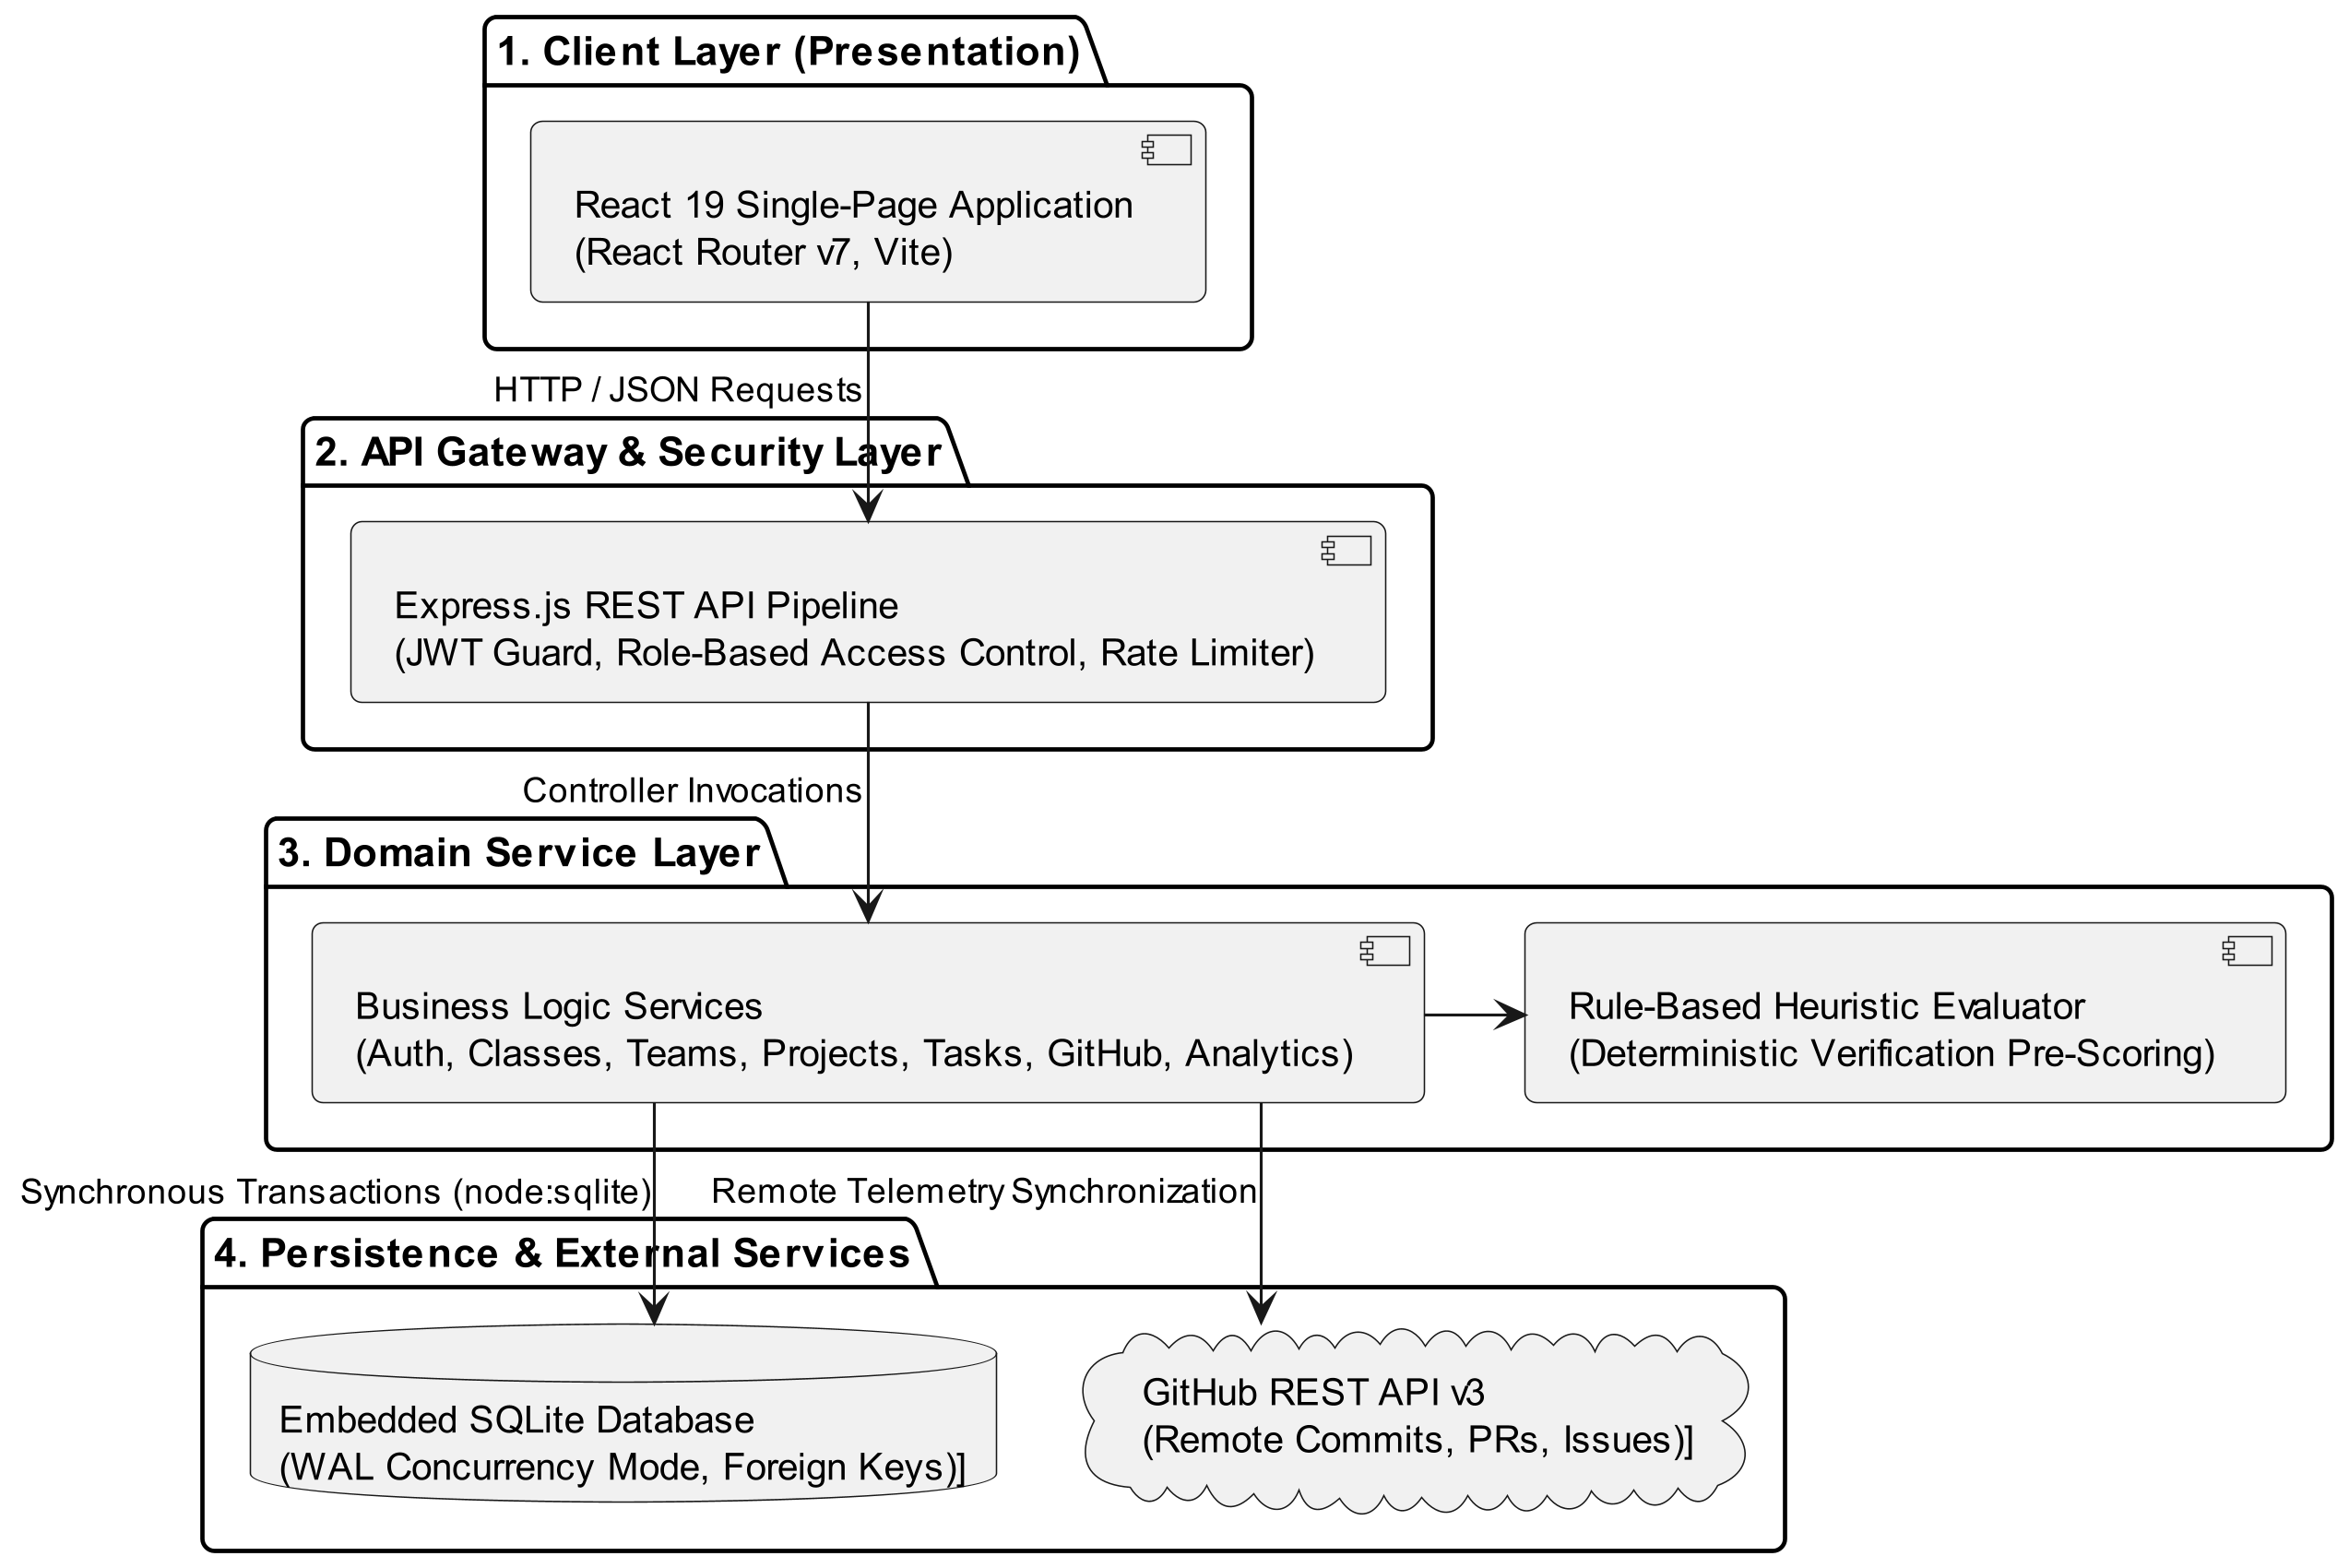
\includegraphics[width=0.82\textwidth]{system_architecture.png}
    \caption{ProjNaN Simplified 4-Tier System Architecture}
    \label{fig:system_architecture}
\end{figure}

Figure~\ref{fig:system_architecture} illustrates the system components:
\begin{itemize}
    \item \textbf{Client Layer}: A responsive Single-Page Application (SPA) built with React 19, React Router v7, and Vite, featuring Kanban boards, telemetry tabs, and velocity graphs.
    \item \textbf{API Gateway Layer}: An Express.js REST API enforcing request sanitization, sliding-window rate limiting, stateless JWT authentication, and role-based access control.
    \item \textbf{Domain Service Layer}: Modular business logic services handling authentication, classes, teams, projects, tasks, telemetry, contributions, and gamification, integrated with the internal rule-based heuristic evaluator.
    \item \textbf{Persistence Layer}: Embedded SQLite storage operating in WAL mode to guarantee ACID transactional consistency, indexed queries, and cascade safety.
\end{itemize}

\begin{figure}[H]
    \centering
    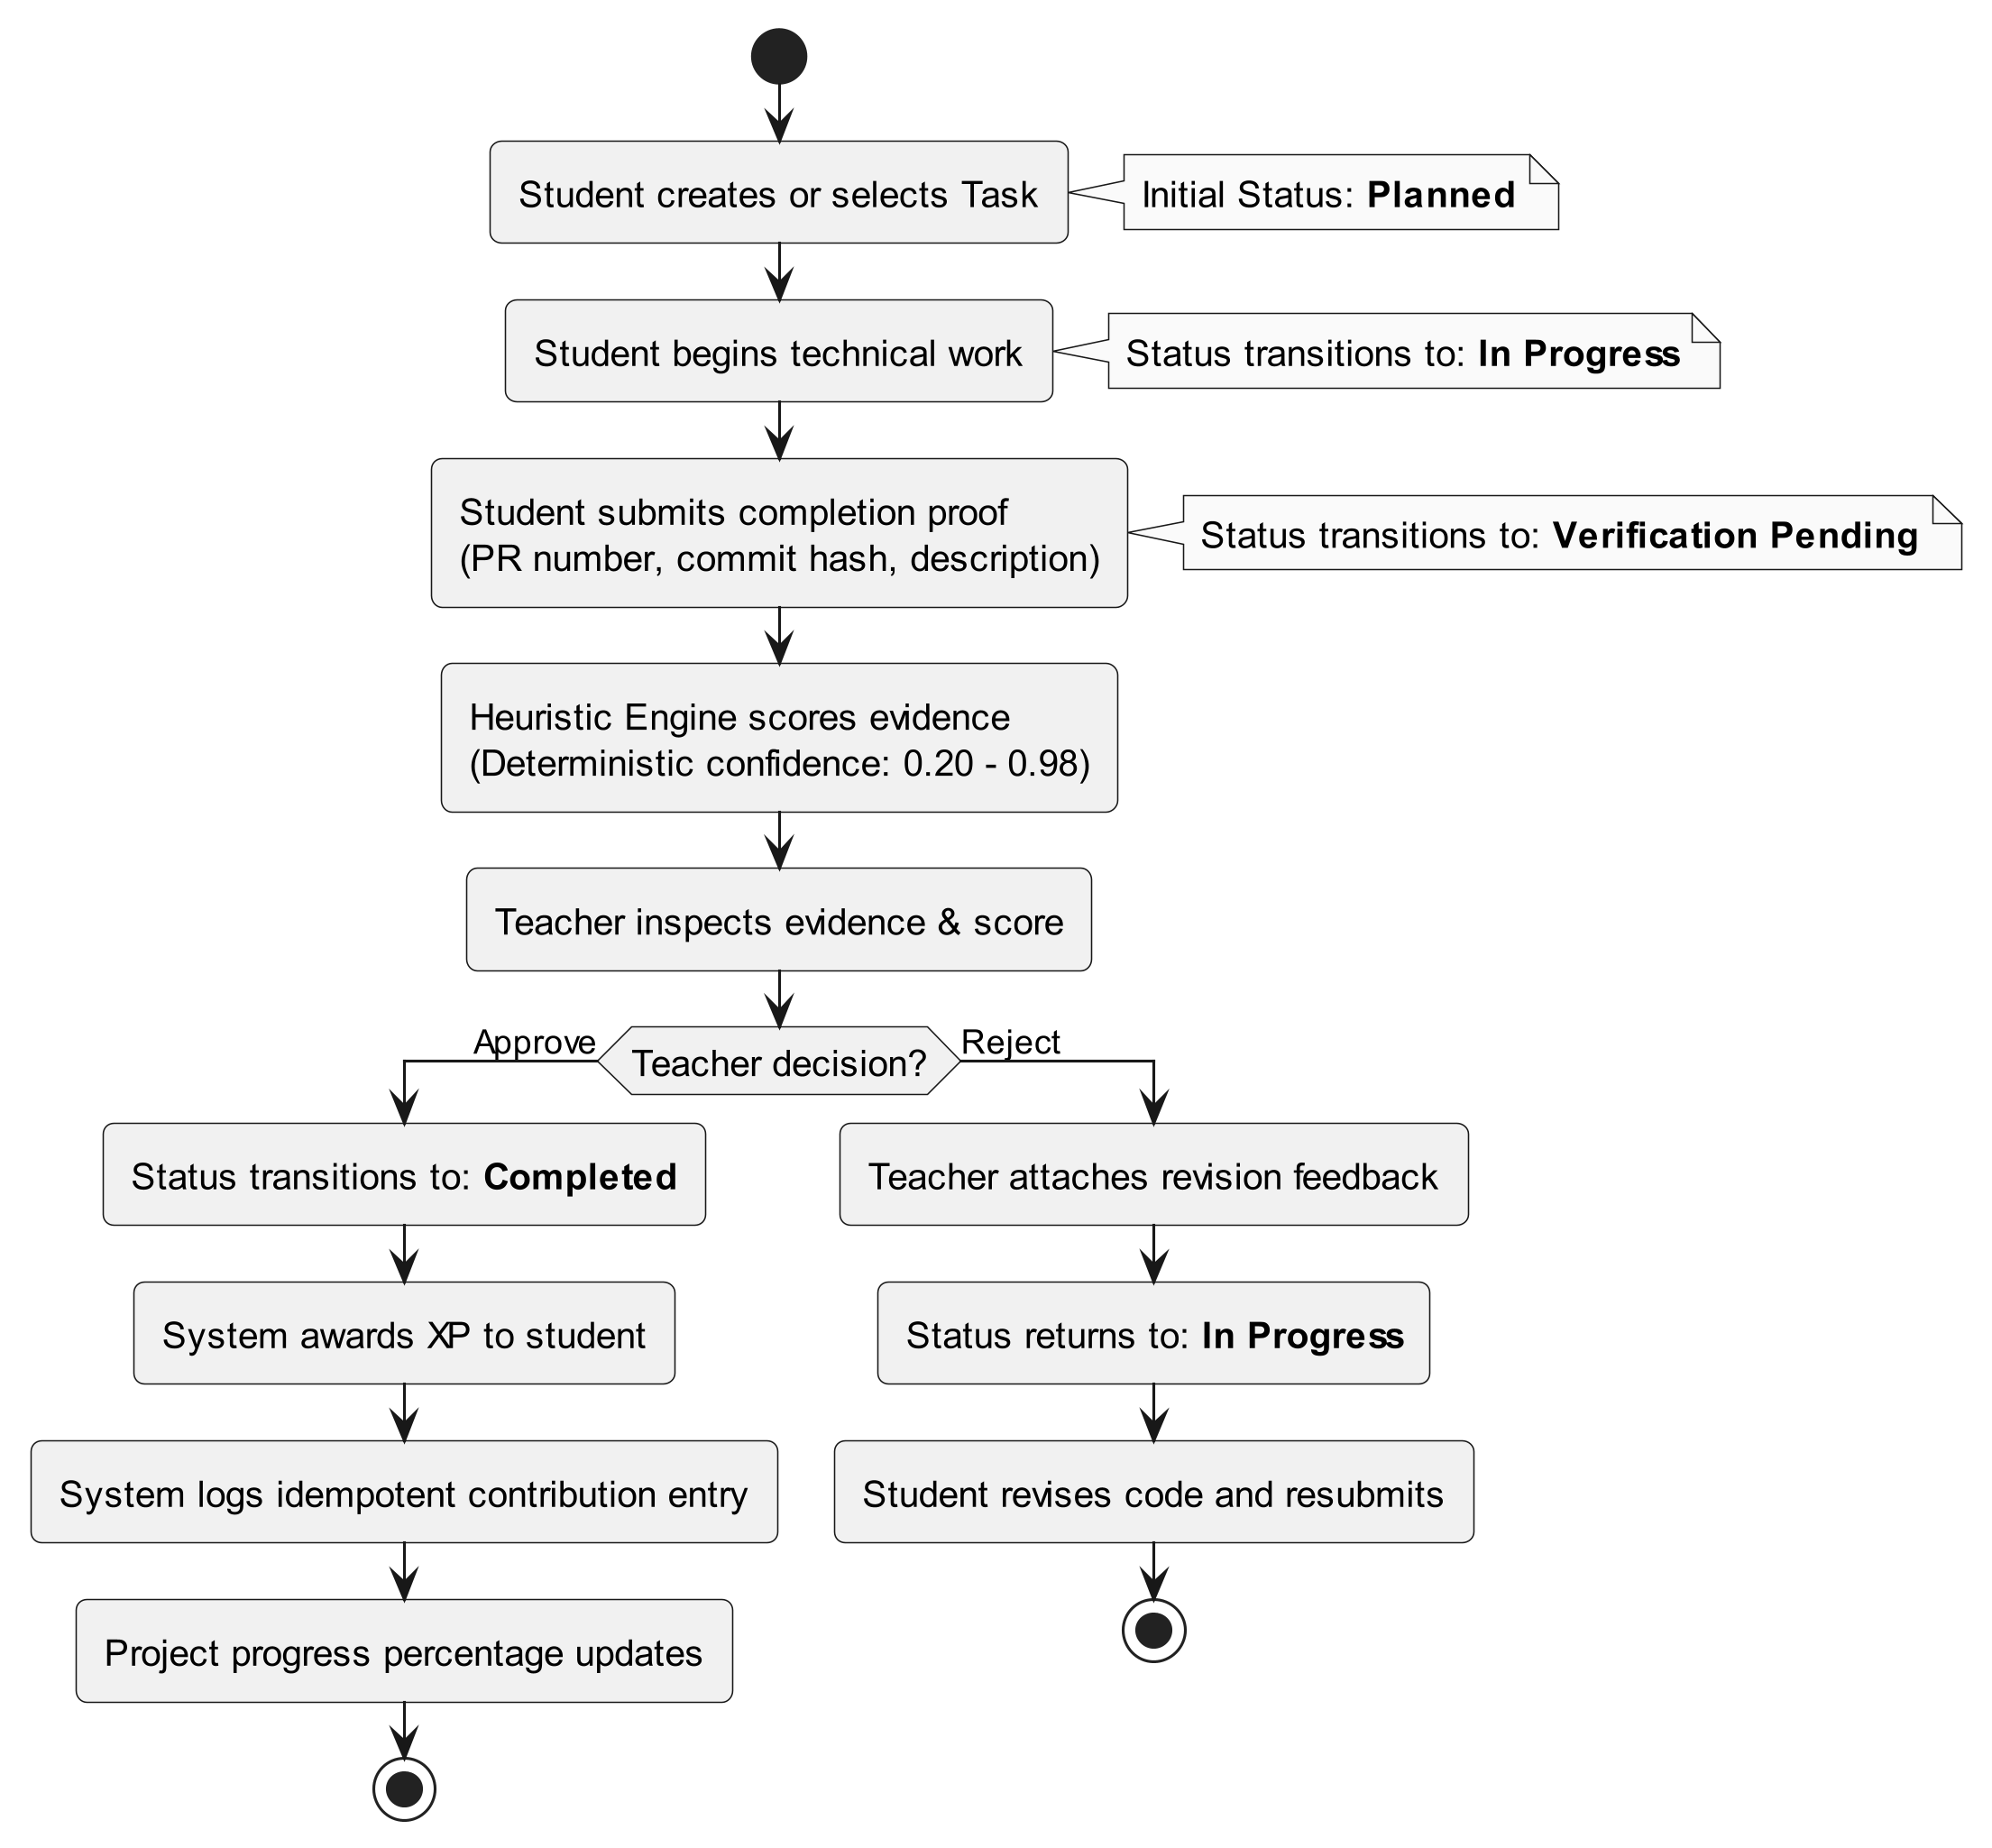
\includegraphics[width=0.62\textwidth]{task_activity.png}
    \caption{Task Verification and Lifecycle Activity Flow}
    \label{fig:task_activity}
\end{figure}

Figure~\ref{fig:task_activity} details the task lifecycle activity flow. Tasks begin in the \texttt{Planned} state and move to \texttt{In Progress} when work starts. Submitting evidence transitions the task to \texttt{Verification Pending} and triggers the rule-based evaluator. The course instructor reviews the evidence and either approves the task (moving it to \texttt{Completed} and awarding XP) or rejects it with feedback (returning it to \texttt{In Progress} for student revision).


%% CHAPTER 3: SYSTEM FEATURES
\chapter{System Features}\label{chap:system_features}

This chapter details the functional features of ProjNaN. All protected endpoints follow standard RESTful error conventions: unauthenticated requests return HTTP 401 Unauthorized, invalid input returns HTTP 400 Bad Request, unauthorized role actions return HTTP 403 Forbidden, and rate-limit violations return HTTP 429 Too Many Requests.

\section{Description and Priority}\label{sec:feature_priority}
The system capabilities are prioritized in Table~\ref{tab:feature_priority}.

\begin{table}[H]
\centering
\begin{tabularx}{\textwidth}{|l|l|c|X|}
    \hline
    \textbf{Module ID} & \textbf{Feature Description} & \textbf{Priority} & \textbf{Primary Actor} \\
    \hline
    \textbf{MOD-01} & User Authentication, Session, and RBAC & High & All Users \\
    \textbf{MOD-02} & Academic Class Scoping and Team Formation & High & Teacher / Student \\
    \textbf{MOD-03} & Project Workspaces and Milestone Tracking & High & Student / Teacher \\
    \textbf{MOD-04} & Task Lifecycle (4-Stage State Machine) & High & Student / Teacher \\
    \textbf{MOD-05} & Heuristic Evidence Evaluation Engine & High & System \\
    \textbf{MOD-06} & Faculty Task Verification and Confirmation & High & Teacher \\
    \textbf{MOD-07} & GitHub Telemetry Synchronization & Medium & Student / System \\
    \textbf{MOD-08} & Idempotent Contribution Ledger \& Analytics & High & System / All Users \\
    \textbf{MOD-09} & Gamification (Weekly Arena \& Leaderboard) & Medium & Student \\
    \textbf{MOD-10} & Pedagogical Feedback (1--5 Star Reviews) & Medium & Teacher \\
    \textbf{MOD-11} & Persistent Notifications \& Project Channels & Low & All Users \\
    \hline
\end{tabularx}
\caption{System Feature Priority Matrix}
\label{tab:feature_priority}
\end{table}

\section{Functional Requirements}\label{sec:functional_requirements}

\subsection{MOD-01: User Authentication, Session Management, and RBAC}
Manages identity lifecycles, role-based authorization, email verification, and password recovery.
\begin{itemize}
    \item \textbf{FR-1.1: Account Registration}: The system shall accept user registration with name, unique username, unique email address, password, and role (\texttt{'teacher'} or \texttt{'student'}). Passwords must contain at least 6 characters including uppercase, lowercase, and numeric digits, hashed using \texttt{bcryptjs} with 10 salt rounds.
    \item \textbf{FR-1.2: Email Verification Token}: Upon registration, the system shall generate a random 64-character hexadecimal verification token and initialize \texttt{email\_verified = 0}.
    \item \textbf{FR-1.3: User Authentication}: The system shall validate login credentials against stored bcrypt hashes and issue an HMAC-SHA256 signed JWT containing \texttt{userId}, \texttt{email}, and \texttt{role}, valid for 7 days.
    \item \textbf{FR-1.4: Password Reset Lifecycle}: The system shall support a two-stage password recovery workflow. Requesting a reset generates a 64-hex token valid for 1 hour. Submitting a compliant new password updates the hash and invalidates the token.
    \item \textbf{FR-1.5: Role-Based Authorization Guard}: The API gateway shall intercept incoming requests using role middleware, rejecting unauthorized role access with HTTP 403 Forbidden.
\end{itemize}

\subsection{MOD-02: Academic Class Scoping and Team Formation}
Provides course scoping by enabling instructors to create classes and allowing students to form collaborative teams.
\begin{itemize}
    \item \textbf{FR-2.1: Class Creation}: Instructors shall create academic classes with a course title and description. The system shall automatically generate a unique alphanumeric class join code (e.g., \texttt{CS101-ABCD}).
    \item \textbf{FR-2.2: Student Self-Enrollment}: Students shall join an academic class by submitting a valid class join code. The system validates the code and adds the student to the class roster.
    \item \textbf{FR-2.3: Class Roster Visibility}: Instructors shall be capable of viewing the complete roster of enrolled students, their enrollment dates, and assigned project teams.
    \item \textbf{FR-2.4: Team Formation}: Students enrolled within a class shall form collaborative teams by specifying a team name, designating the creator as initial team leader.
\end{itemize}

\subsection{MOD-03: Project Workspaces and Milestone Tracking}
Governs project definitions, progress calculations, and milestone deadlines.
\begin{itemize}
    \item \textbf{FR-3.1: Project Workspace Instantiation}: Each team shall establish a project workspace categorized under their enrolled class, containing project title, description, goals, and topical tags.
    \item \textbf{FR-3.2: Milestone Definition}: Projects shall contain milestones with titles, descriptions, target due dates, and completion XP values (\texttt{xp\_reward}, default 100 XP).
    \item \textbf{FR-3.3: Dynamic Progress Calculation}: The system shall dynamically compute overall project completion progress as an integer percentage:
    \begin{equation}
        \text{Progress} = \left( \frac{N_{\text{completed tasks}}}{N_{\text{total tasks}}} \right) \times 100
    \end{equation}
    The calculated percentage updates synchronously upon any task status transition.
\end{itemize}

\subsection{MOD-04: Task Management and 4-Stage State Lifecycle}
Enforces a structured 4-stage state machine across units of project work.
\begin{itemize}
    \item \textbf{FR-4.1: Task Creation}: Team members shall create tasks with attributes: \texttt{title}, \texttt{description}, \texttt{assigned\_to\_id}, \texttt{milestone\_id}, \texttt{priority} (\texttt{'low'}, \texttt{'medium'}, \texttt{'high'}, \texttt{'urgent'}), \texttt{task\_type} (\texttt{'daily'}, \texttt{'weekly'}, \texttt{'monthly'}), \texttt{deadline}, and \texttt{xp\_value} (default 50 XP). Initial status is set to \texttt{'Planned'}.
    \item \textbf{FR-4.2: Work Inception}: When an assigned student begins implementation, task status transitions from \texttt{'Planned'} to \texttt{'In Progress'}.
    \item \textbf{FR-4.3: Evidence Submission Gate}: A task cannot transition directly from \texttt{'In Progress'} to \texttt{'Completed'}. The student must submit non-empty technical evidence text to trigger transition to \texttt{'Verification Pending'}.
    \item \textbf{FR-4.4: Task Assignment Notification}: Assigning a task to a team member shall automatically generate an in-app notification for that user.
\end{itemize}

\subsection{MOD-05: Evidence Submission and Rule-Based Heuristic Evaluation}
Analyzes student-submitted evidence using deterministic pattern matching and local repository cross-referencing.
\begin{itemize}
    \item \textbf{FR-5.1: Evidence Text Validation}: Submitting completion evidence requires non-empty text. Empty submissions return HTTP 400 Bad Request.
    \item \textbf{FR-5.2: Heuristic Confidence Evaluation}: The internal engine evaluates evidence text through a deterministic rule-based formula:
    \begin{equation}
        S_{\text{confidence}} = \min\left(0.98, \, \max\left(0.20, \, S_{\text{base}} + \delta_{\text{len}} + \delta_{\text{PR}} + \delta_{\text{commit}} + \delta_{\text{test}}\right)\right)
    \end{equation}
    where $S_{\text{base}} = 0.50$, length bonus $\delta_{\text{len}} = 0.15$ ($>30$ characters), PR bonus $\delta_{\text{PR}} = +0.25$ (matched in \texttt{github\_activities}) or $+0.10$ (regex pattern cited), commit SHA bonus $\delta_{\text{commit}} = +0.25$ (matched in database) or $+0.10$ (regex pattern cited), and test outcome bonus $\delta_{\text{test}} = +0.10$. Final score is clamped between $0.20$ and $0.98$ (typically $0.50$ to $0.90$).
    \item \textbf{FR-5.3: Heuristic Explanation Compilation}: The system shall construct human-readable explanatory tags detailing the rationale for the calculated score, formatted as \texttt{AI Verification (<Score>\%): <reasons>} (for example: ``\texttt{AI Verification (90\%):} Detailed descriptive summary provided; Verified pull request \#12 linked in repository'').
    \item \textbf{FR-5.4: Verification Persistence}: The system shall persist the evaluation record with status \texttt{'suggested'} linked to the task.
\end{itemize}

\subsection{MOD-06: Faculty Task Verification and Confirmation}
Empowers course instructors to make authoritative verification decisions on submitted tasks.
\begin{itemize}
    \item \textbf{FR-6.1: Role Guard Enforcement}: Only authenticated users with \texttt{role = 'teacher'} are permitted to invoke the verification endpoint. Student attempts return HTTP 403 Forbidden.
    \item \textbf{FR-6.2: Approval Decision Execution}: When an instructor approves a task:
    \begin{enumerate}
        \item Task status updates to \texttt{'Completed'} and \texttt{verification\_status = 'verified'}.
        \item Verification record transitions to \texttt{'confirmed'}.
        \item The assigned student's profile is credited with \texttt{xp = xp + task.xp\_value} and contribution points.
        \item An entry is inserted into the idempotent \texttt{contributions} ledger with \texttt{external\_id = 'task:<id>'}.
        \item Overall project progress percentage is recalculated.
        \item A persistent notification is delivered to the student.
    \end{enumerate}
    \item \textbf{FR-6.3: Rejection Decision Execution}: When an instructor rejects a task:
    \begin{enumerate}
        \item Task status returns to \texttt{'In Progress'} and its \texttt{verification\_status} updates to \texttt{'rejected'}.
        \item Verification record updates to \texttt{'rejected'}, appending the teacher's feedback notes.
        \item No XP or contribution points are awarded.
        \item A notification detailing required revisions is dispatched to the student.
    \end{enumerate}
\end{itemize}

\subsection{MOD-07: External GitHub Telemetry Synchronization}
Synchronizes remote commits, pull requests, and issues from the GitHub REST API v3 into local relational storage.
\begin{itemize}
    \item \textbf{FR-7.1: Repository Connection}: A project workspace shall connect to a remote GitHub repository by specifying a valid repository URL and an optional Personal Access Token (PAT).
    \item \textbf{FR-7.2: Remote Endpoint Ingestion}: Triggering synchronization invokes the GitHub REST API v3 to fetch recent commits, pull requests, and issues.
    \item \textbf{FR-7.3: Activity Ingestion and Deduplication}: Fetched items are normalized and inserted into \texttt{github\_activities}, recording commit SHAs, PR numbers, author logins, and timestamps.
    \item \textbf{FR-7.4: Network Fault Resilience}: In the event of network timeouts, DNS resolution failures, or GitHub rate limiting, the synchronization pipeline shall catch exceptions gracefully, set repository sync status to \texttt{'error'}, and prevent application crashes.
\end{itemize}

\subsection{MOD-08: Idempotent Contribution Ledger and Team Analytics}
Maintains an idempotent activity ledger that prevents double-counting across repeated sync passes and computes team velocity and relative effort distribution.
\begin{itemize}
    \item \textbf{FR-8.1: Idempotency Key Enforcement}: Every contribution record requires a deterministic external reference key (\texttt{external\_id}), such as \texttt{commit:<sha>}, \texttt{pr:<repo>:<num>}, or \texttt{task:<taskId>}. If an entry with an identical \texttt{external\_id} exists, insertion is safely skipped without duplicate XP attribution.
    \item \textbf{FR-8.2: Author Matching Logic}: When repository activity is ingested, the system attempts to match GitHub author logins or commit author names against registered project team members. Unmatched commits remain stored in \texttt{github\_activities} but do not enter the contribution ledger.
    \item \textbf{FR-8.3: Relative Effort Share Calculation}: The analytics engine calculates each team member's relative contribution share ($P_i$):
    \begin{equation}
        P_i = \left( \frac{C_i}{\sum_{k=1}^N C_k} \right) \times 100
    \end{equation}
    where $C_i$ represents member $i$'s total verified contribution count and $N$ is the number of active team members.
    \item \textbf{FR-8.4: 14-Day Velocity Sparkline}: The system aggregates verified contributions across a rolling 14-day window to compute daily activity volume and XP velocity curves for frontend visualization.
\end{itemize}

\subsection{MOD-09: Gamification, Weekly Arena, and Leaderboard}
Incentivizes technical engagement through coding challenges, achievement badges, and XP-driven student ranks.
\begin{itemize}
    \item \textbf{FR-9.1: Arena Challenge Catalog}: The platform hosts coding challenges categorized by difficulty (\texttt{'Easy'}, \texttt{'Medium'}, \texttt{'Hard'}) with assigned XP rewards (e.g., 150 XP).
    \item \textbf{FR-9.2: Challenge Submission}: Students accept and submit challenge solutions alongside verification evidence, earning XP upon acceptance.
    \item \textbf{FR-9.3: Gamified Rank Tiers}: Students progress through defined achievement ranks based on cumulative XP:
    \begin{itemize}
        \item \textbf{Novice}: $0 - 249$ XP
        \item \textbf{Explorer}: $250 - 499$ XP
        \item \textbf{Contributor}: $500 - 999$ XP
        \item \textbf{Expert}: $1000 - 1999$ XP
        \item \textbf{Master}: $\ge 2000$ XP
    \end{itemize}
    \item \textbf{FR-9.4: Class and Global Leaderboard}: The system renders ranked leaderboards displaying total XP, earned badges, and completed challenges.
\end{itemize}

\subsection{MOD-10: Pedagogical Feedback and 1--5 Star Reviews}
Enables instructors and peers to attach qualitative feedback and standardized ratings to student projects.
\begin{itemize}
    \item \textbf{FR-10.1: Instructor Project Review}: Faculty mentors shall submit structured evaluations containing a 1--5 star integer rating and qualitative commentary regarding architecture, code quality, and collaboration.
    \item \textbf{FR-10.2: Peer Feedback}: Team members shall provide constructive feedback on peer contributions.
    \item \textbf{FR-10.3: Review Notifications}: Submitting feedback shall generate an immediate notification for all members of the target project team.
\end{itemize}

\subsection{MOD-11: Persistent Notifications and Project Channel Discussion}
Provides asynchronous in-app notifications and project-scoped discussion channels.
\begin{itemize}
    \item \textbf{FR-11.1: Event-Driven Alerts}: The system generates persistent notifications for task assignments, verification approvals/rejections, milestone deadlines, and feedback submissions.
    \item \textbf{FR-11.2: Read State Management}: Unread alerts are flagged with an unread badge and can be marked as read individually or in bulk.
    \item \textbf{FR-11.3: Project Discussion Channels}: Each project workspace contains dedicated chat channels (e.g., \texttt{\#general}, \texttt{\#dev}) for team communication.
\end{itemize}


%% CHAPTER 4: OTHER NONFUNCTIONAL REQUIREMENTS
\chapter{Other Nonfunctional Requirements}\label{chap:nonfunctional_requirements}

\section{Performance Requirements}\label{sec:performance}
\begin{itemize}
    \item \textbf{NFR-1.1: Database Query Latency (Design Target)}: Local SQLite queries for indexed primary keys (user lookups, task status queries) are targeted to execute in under 10 milliseconds under nominal laboratory workloads.
    \item \textbf{NFR-1.2: API Endpoint Response Time (Design Target)}: Standard CRUD endpoints are targeted to return responses within 200 milliseconds under nominal concurrent student usage.
    \item \textbf{NFR-1.3: Telemetry Synchronization Duration (Design Target)}: Repository synchronization over a stable Internet connection is targeted to ingest recent commits and pull requests within 5 seconds.
    \item \textbf{NFR-1.4: Frontend Bundle Footprint (Verified Target)}: Production Single-Page Application assets are targeted to remain under $450$ kB uncompressed ($\le 125$ kB gzip-compressed) to ensure rapid loading on campus networks. An empirical production build (\texttt{npm run build} via Vite) was verified: the compiled JavaScript client bundle is exactly $412.44$ kB ($113.60$ kB gzip-compressed), and the compiled stylesheet bundle is $29.64$ kB ($6.30$ kB gzip-compressed), fully satisfying the performance target.
\end{itemize}

\section{Security Requirements}\label{sec:security}
\begin{itemize}
    \item \textbf{NFR-2.1: Password Hashing}: Raw passwords shall never be stored in plain text. Hashing must employ \texttt{bcryptjs} with a minimum of 10 salt rounds.
    \item \textbf{NFR-2.2: Cross-Site Scripting (XSS) Sanitization}: The application pipeline incorporates recursive sanitization middleware that strips script injection vectors from all incoming request bodies.
    \item \textbf{NFR-2.3: Authentication Rate Limiting}: To mitigate brute-force credential guessing, an in-memory sliding-window rate limiter restricts authentication attempts to a maximum of 15 requests per 15-minute window per IP address, responding with HTTP 429 upon breach.
    \item \textbf{NFR-2.4: RBAC Enforcement}: Crucial administrative operations (approving task verifications, creating classes) strictly enforce teacher authorization, guaranteeing that student attempts return HTTP 403 Forbidden.
    \item \textbf{NFR-2.5: Token Expiration and Isolation}: Password reset tokens are constrained to a strict 1-hour expiration window; JWT session tokens expire after 7 days.
    \item \textbf{NFR-2.6: Transactional Atomicity}: Multi-table state mutations (e.g., confirming task verification, updating task status, crediting user XP, and logging the contribution ledger) execute within atomic database transactions. In the event of an unhandled runtime error, changes automatically roll back. The SQLite engine operates in Write-Ahead Logging (WAL) mode, providing crash resilience during unexpected process termination.
\end{itemize}

\section{Software Quality Attributes}\label{sec:quality_attributes}
\begin{itemize}
    \item \textbf{Reliability}: The platform delivers high availability through graceful fault tolerance. Network errors during GitHub synchronization are caught without crashing the application server.
    \item \textbf{Maintainability}: The backend follows a clean, modular service-oriented architecture (controllers, services, middleware, database models) separating concerns.
    \item \textbf{Usability}: The interface minimizes cognitive load by surfacing heuristic confidence tags and color-coded statuses, allowing instructors to evaluate student tasks quickly.
    \item \textbf{Testability}: The functional stability and security guards of ProjNaN are verified through 52 automated tests executed by the Node.js native test runner (\texttt{node:test}). All 52 tests pass with 100\% success across authentication (16 tests), core workflow (23 tests), gamification (6 tests), and security guards (7 tests).
\end{itemize}

\section{Business Rules}\label{sec:business_rules}
\begin{itemize}
    \item \textbf{BR-1: Verified Task Completion}: A task cannot transition to \texttt{'Completed'} unless an authenticated course instructor (\texttt{teacher}) explicitly confirms verification. Student self-completion is prevented, and no unverified administrative override exists in the system.
    \item \textbf{BR-2: Single Active Repository Link}: Each project workspace can link to at most one remote GitHub repository at any given time (\texttt{UNIQUE(project\_id)} constraint in \texttt{repositories}).
    \item \textbf{BR-3: Idempotent Ledger Integrity}: Contribution XP can be granted for a specific Git commit or completed task at most once. Idempotency is enforced by the \texttt{external\_id} index in the \texttt{contributions} table.
    \item \textbf{BR-4: Class Join Code Uniqueness}: Class codes must remain globally unique across the institution to prevent ambiguous course enrollment.
\end{itemize}


%% CHAPTER 5: OTHER REQUIREMENTS
\chapter{Other Requirements}\label{chap:other_requirements}

\section{Maintenance Requirements}\label{sec:maintenance}
As software engineering pedagogical practices evolve, ProjNaN requires ongoing maintenance:
\begin{itemize}
    \item \textbf{Schema Evolution}: Future relational migrations must execute via transactional migration scripts, ensuring backward compatibility.
    \item \textbf{Database Archival}: At the conclusion of each academic semester, completed classes and associated telemetry can be archived to prevent database file bloat.
\end{itemize}

\section{Future Roadmap}\label{sec:future_roadmap}
The following architectural extensions represent planned future enhancements:
\begin{enumerate}
    \item \textbf{LLM Semantic Code Diff Review}: Integrating Large Language Model (LLM) agents to analyze Git code diffs semantically for architectural adherence and code quality.
    \item \textbf{Full-Duplex WebSocket Infrastructure}: Transitioning project channel chat from HTTP REST polling to persistent WebSockets for real-time messaging.
    \item \textbf{Cross-Project Plagiarism Detection}: Integrating source-code similarity algorithms (e.g., automated MOSS API adapters) to detect unauthorized code copying between team repositories.
\end{enumerate}

\end{document}
